\documentclass[12pt,titlepage]{article}

\usepackage{geometry}
\geometry{
    a4paper,
    total={210mm,297mm},
    left=20mm,
    right=20mm,
    top=20mm,
    bottom=20mm,
}

	
\usepackage[]{subcaption}

\usepackage{pdflscape}

% Polski
\usepackage[]{polski} 
\usepackage[polish]{babel}

%do tabel
\usepackage{multirow}

% Pierwszy akapit - wcięty
\usepackage[]{indentfirst}

% Matematyka
\usepackage[]{amsfonts}

\usepackage[]{amsmath}

% Formatowanie
\usepackage{ragged2e}

% Tytuły sekcji
\usepackage{titlesec}
%\titleformat{\section}[block]{\Large\bfseries}{}{1em}{}

% <=
\usepackage{amssymb}

% eps
\usepackage{graphicx}
% \usepackage{subfigure}

% Tabele
\usepackage{array}

\usepackage[style=czech]{csquotes}

\renewcommand*{\thesubsubsection}{}

\usepackage{hyperref}
\hypersetup{
    colorlinks,
    citecolor=black,
    filecolor=black,
    linkcolor=black,
    urlcolor=black
}

\usepackage[numbered]{matlab-prettifier}
\lstset{
    literate={ą}{{\k{a}}}1
    {Ą}{{\k{A}}}1
    {ę}{{\k{e}}}1
    {Ę}{{\k{E}}}1
    {ó}{{\'o}}1
    {Ó}{{\'O}}1
    {ś}{{\'s}}1
    {Ś}{{\'S}}1
    {ł}{{\l{}}}1
    {Ł}{{\L{}}}1
    {ż}{{\.z}}1
    {Ż}{{\.Z}}1
    {ź}{{\'z}}1
    {Ź}{{\'Z}}1
    {ć}{{\'c}}1
    {Ć}{{\'C}}1
    {ń}{{\'n}}1
    {Ń}{{\'N}}1
}

\title{

\includegraphics[scale=0.75]{img/politechnika_sl_logo_bw_poziom_pl.eps}\\
\textbf{Wydział Automatyki, Elektroniki\\
i Informatyki}\\
\vspace*{1cm}
Systemy Interaktywne i Multimedialne \\ Projekt \\ Detekcja emocji w głosie

\vspace*{5cm}
}
\author{
Natalia Stręk
Jakub Kula,
Paweł Wójtowicz,
} 
\date{Gliwice 2023}

\begin{document}

\maketitle

% \tableofcontents

\newpage
\section{Analiza wyników i wnioski}
% Cele i zadania z okresu objętego sprawozdaniem, których realizację już podjęto. Należy odnieść się do zaakceptowanego dokumentu Informacje o realizowanym projekcie (ok 100 słów)\\
\subsection{Cele i zadania z okresu maczec-kwiecień}
Cele wyznaczone na okres marzec-kwiecień obejmowały przede wszystkim zgłębienie wiedzy na temat przetwarzania plików audio oraz zidentyfikowanie cech, które można wykorzystać w procesie nauki modelu uczenia maszynowego. W szczególności chodziło o poznanie technik ekstrakcji cech i analizy dźwięku, aby lepiej zrozumieć, jakie elementy są istotne z punktu widzenia efektywności modelu.
Następnym etapem było stworzenie odpowiedniego skryptu do przetwarzania danych, który umożliwiłby ekstrakcję wcześniej zidentyfikowanych charakterystycznych cech. Ostatnim postawionym celem na ten okres było stworzenie modelu sieci neuronowej posiadajacej minium 50\% dokładności, który by służył jako model referencyjny do którego będą porónywane kolejne stworzone modele.\\

% Opis zadań przyjętych do realizacji w okresie objętym sprawozdaniem w odniesieniu do poszczególnych etapów pracy. Które z zadań zostały wykonane? Które z zadań są realizowane? Jaki jest procentowy postęp prac? Ile przeznaczono czasu na wykonanie poszczególnych zadań? (ok 300 słów)\\
\subsection{Opis zadań przyjętych do realizacji}
\subsubsection{Zgromadzenie i przetworzenie danych}
Aby stworzyć model klasyfikacji emocji z dźwięku, wykorzystano dane z dwóch źródeł: Ravdess i TESS. Pierwotnie planowano wykorzystać wyłącznie zbiór Ravdess, jednak w celu zwiększenia różnorodności i objętości danych, do projektu włączono również zbiór TESS.
\subsubsection{Wybór oraz ekstrakcja cech}
W trakcie okresu marzec-kwiecień zostały wybrane cechy dziwięku które zostały użyte jako wejścia do sieci neuronowej. Wybrane wejścia do sieci to:
\begin{itemize}
    \item \textbf{Chroma STFT}: Reprezentacja częstotliwości dźwięku w sposób związany z tonalnością, używana w analizie akordów i melodii.
    \item \textbf{MFCC}: Kompaktowa reprezentacja dźwięku, oparta na skali melowej, często stosowana w rozpoznawaniu mowy i dźwięku.
    \item \textbf{Root Mean Square Value}: Średnia wartość kwadratu sygnału dźwiękowego, stosowana do oceny głośności.
    \item \textbf{Spectral Centroid}: Średnia częstotliwość w spektrum dźwięku, służy do oceny barwy dźwięku.
    \item \textbf{Spectral Spread}: Mierzona rozpiętość częstotliwości w spektrum dźwięku, informuje o jego różnorodności częstotliwości.
    \item \textbf{Spectral Flux}: Miara zmienności spektrum dźwięku w czasie, używana w analizie dynamiki dźwięku.
    \item \textbf{Spectral Roll-Off}: Częstotliwość, poniżej której kumulatywna energia spektrum jest mniejsza niż określony procent całkowitej energii.
    \item \textbf{Chroma Vector}: Wektor reprezentujący rozkład mocy dźwięku w chromie, używany w analizie harmonicznej.
    \item \textbf{MelSpectrogram}: Spektrogram dźwięku, gdzie skala częstotliwości jest przekształcona na skalę melową, co odzwierciedla sposób, w jaki ludzkie ucho percepcyjnie odbiera dźwięki.
\end{itemize}
W celu zmniejszenia wymiarowości danych, została wyciągnięta średnia z każdej cechy z każdego segmentu czasowego.\\
\subsubsection{Wybór architektury sieci oraz trenowanie modelu}
W realizowanym projekcie wykorzystano konwolucyjne sieci neuronowe (CNN), architektura ta wykorzystuje takie warstwy jak konwolucyjne do wykrywania wzorców, poolingowe do redukcji wymiarów oraz z warst gęstych do końcowej klasyfikacji.

Została także wytrenowana sieć która osiąga 68\% dokładności. Jendak podczas testów na zbiorze testowym osiąga ta sieć dokładność rzędu 45\%, co wskazuje na znaczącą różnicę w wydajności między zbiorem uczącym a testowym.\\

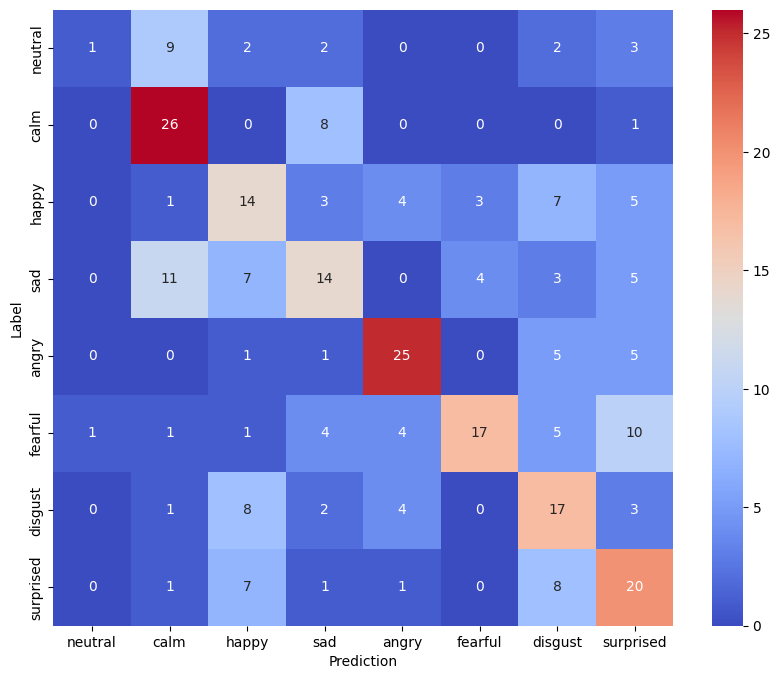
\includegraphics[width=\linewidth]{img/error_matrix.png}

Do tej pory przeprowadzono wybór danych, ich przetwarzanie oraz ekstrakcję cech. Dodatkowo dokonano doboru architektury sieci neuronowej oraz stworzono modele uczenia maszynowego, które klasyfikują nagrania głosowe. Modele zostały poddane ocenie i walidacji w celu sprawdzenia ich dokładności i skuteczności w przewidywaniu oraz klasyfikacji. Ze względu na nieustanne poszukiwanie coraz doskonalszych modeli, proces ten pozostaje w ciągłej realizacji, dążenie do optymalizacji modelu wymaga ciągłego testowania oraz wprowadzania ulepszeń w celu osiągnięcia jak najskuteczniejszego modelu w klasyfikacji nagrań. Na ten moment szacujemy, że około 60\% projektu zostało już zrealizowane.

% Czy projekt realizowany jest zgodnie z harmonogramem? Jeśli nie, podać przyczyny opóźnień w odniesieniu do etapów pracy oraz opisać działania naprawcze mających na celu osiągnięcie celów i wyników projektu\\
Projekt jest realizowany zgodnie z harmonogramem.\\

% Czy wprowadzono jakieś znaczące zmiany do zrealizowanych działań lub w składzie zespołu? Jeśli tak, opisać jakie oraz podać ich wpływ na realizację projektu.
\subsection{Dodatkowy zbiór danych}
Wprowadzono następujące zmiany w założeniach projektu:
Dodano kolejny zbiór nagrań. Zbiór TESS  Toronto emotional speech set posiada aż 2800 nagrań podzielonych na 6 klas.  Do projektu użytko tylko nagrań audio. Klasy to: neutral, happy, sad, angry, fearful, surprise i disgust. Zbiór TESS nie posiada emocji calm który posiadał zbiór Ravdess. Wykorzystanie dodatkowego zbioru pozwala na wprowadzenie większej różnorodności dlatego też model ten może lepiej osiągąć lepszą dokładność w klasyfikacji nowych danych.\\
Kolejną zmianą jest zmniejszenie długości nagrań głosowych do jednej sekundy. Zostało to zastosowane ze względu na to, że wszystkie nagrania muszą mieć taką samą długość, a dane z nowego zbioru są znacząco krótsze. Dane ze zbioru Ravdess zostały użyte od 0.6s do 1.6s.

\end{document}